\section{Evaluation}

\hspace{\parindent}
 We do not implement a full-fledged automated theorem proving system in this work; however, tasks such as
\textit{step completion} would very likely be a central part of any practical system involving large language models
in formal reasoning \cite{proofwaala}


For our experiment, we selected theorems whose proofs in Metamath notation contain between 5 and 25 steps — short
enough to be manageable and computationally efficient, yet long enough to demonstrate meaningful structure. The
resulting dataset includes over 6,000 theorems, each of them had a proof in the Lemmon notation (generated by
\texttt{metamath.exe} with the \texttt{/lemmon/renumber} arguments) and our proposed notation (only proof steps on
Python,
without \texttt{import} statements. Check out \href{https://github.com/kamushekp/metamath2py}{GitHub} for more details.)
For each proof, we randomly selected a step from the second half of
the sequence, removed it, and truncated the proof at that point. The model \textit{gpt-4.1-mini-2025-04-14} was then asked to complete the missing step, given the truncated version.


To evaluate the quality of predictions, we employed the \textit{LLM-as-a-judge} paradigm with a a
\textit{single answer grading} setup \cite{llmjudge}, using the same
model to act as a grader. The model was shown both the task, the expected and the generated
step, and asked to assign a score from 0 to 5 based on structural correctness, syntactic validity, and overall
similarity to the reference.

\begin{figure}[h]
  \centering
  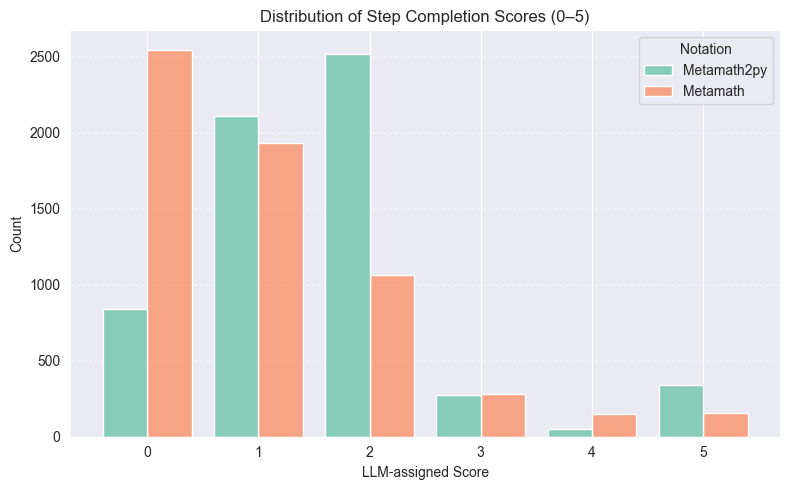
\includegraphics[scale=0.5]{step_completion_score.png}
  \caption{LLM-as-a-judge step completion scores.}
  \label{fig:fig1}
\end{figure}

Figure \ref{fig:fig1} shows the distribution of LLM-assigned scores (ranging from 0 to 5, where 5 is better)
evaluating
the
quality of
predicted next proof steps. Python-based representations demonstrate significantly better results compared to the original notation. Most Metamath-based completions received low scores (0 or 1), indicating the model's difficulty in interpreting symbolic notation without additional structural cues. In contrast, Python proofs exhibit a more balanced distribution, peaking at score 2 and with a noticeable portion receiving high scores (3–5).


\begin{figure}[H]
  \centering
  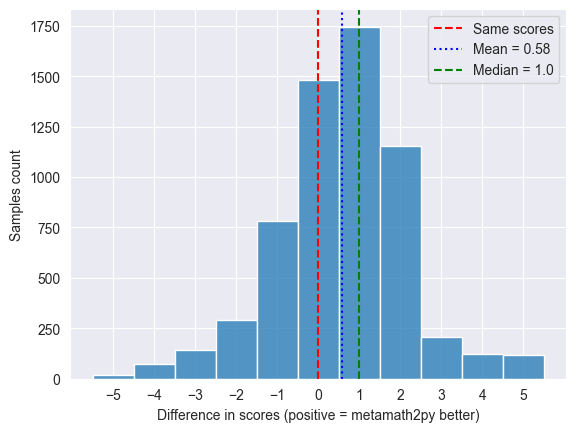
\includegraphics[scale=0.5]{scores_diff.png}
  \caption{Histogram of LLM-assigned score differences.}
  \label{fig:fig2}
\end{figure}


It is useful to compare the change in scores for each proof when the notation changes. Figure \ref{fig:fig2} shows
histogram of
LLM-assigned score differences between the Python-style proofs (metamath2py) and the
original notation. Positive values indicate samples where Metamath2py received higher scores. The
distribution is slightly skewed toward positive values, with a mean of 0.58 and median of 1.0, suggesting improved
step completion quality. The red dashed line marks equal scores; blue and green lines indicate
the mean and median difference, respectively.


This supports the hypothesis that translating formal proofs into a structured and more familiar format—such as Python code—makes it easier for language models to reason about them. Even without specialized adaptation to the task or notation, LLMs are more successful at generating the next proof step when working with representations aligned with their training distribution.



